%% METADATA
%% subject-code: 4311102
%% subject-name: Fundamentals of Electronics
%% semester: 1
%% examination: Summer-2023
%% date: 31-07-2023
%% description: Solution guide for Fundamentals of Electronics Summer 2023 examination
%% tags: study-material, solutions, gtu, 4311102, electronics
%% END METADATA

\documentclass{article}

% content/resources/templates/preamble.tex
\usepackage[margin=0.6in]{geometry}
\author{Milav Dabgar}
\usepackage{amsmath,amssymb,amsthm}
\usepackage{booktabs}
\usepackage{multirow}
\usepackage{xcolor}
\usepackage{tcolorbox}
\tcbuselibrary{breakable,skins}
\usepackage[colorlinks=true,linkcolor=blue]{hyperref}
\usepackage{titlesec}
\usepackage{enumitem}
\usepackage{tikz}
\usepackage{pgfplots}
\usepackage{circuitikz}
\usepackage[version=4]{mhchem}
\usepackage{longtable}
\usepackage{array}
\usepackage{float}
\usepackage{caption}
\usepackage{listings}

\lstset{
  basicstyle=\small\ttfamily,
  breaklines=true,
  breakatwhitespace=false,
  postbreak=\mbox{\textcolor{red}{$\hookrightarrow$}\space},
  float=false,
  numbers=left,
  numberstyle=\tiny\color{gray},
  numbersep=10pt,
  xleftmargin=2em,
  keywordstyle=\color{blue},
  commentstyle=\color{green!60!black},
  stringstyle=\color{purple},
  backgroundcolor=\color{gray!5},
  showstringspaces=false,
  tabsize=2,
  captionpos=b,
  keepspaces=true,
  columns=flexible
}

\pgfplotsset{compat=1.18}
\usetikzlibrary{shapes,arrows,positioning,calc,patterns,decorations.pathmorphing,decorations.markings,arrows.meta}

% Color scheme
\definecolor{headcolor}{RGB}{0,102,204}
\definecolor{keycolor}{RGB}{220,20,60}
\definecolor{solutioncolor}{RGB}{34,139,34}
\definecolor{mnemoniccolor}{RGB}{148,0,211}
\definecolor{codecolor}{RGB}{0,0,100}

% Spacing
\setlength{\parskip}{3pt}
\setlist[itemize]{nosep}
\setlist[enumerate]{nosep}

% Title formatting
\titleformat{\section}{\Large\bfseries\color{headcolor}}{\thesection}{1em}{}
\titleformat{\subsection}{\large\bfseries\color{headcolor}}{\thesubsection}{1em}{}

% Pandoc tightlist compatibility
\providecommand{\tightlist}{%
  \setlength{\itemsep}{0pt}\setlength{\parskip}{0pt}}

% Pandoc longtable compatibility
\newcounter{none}
\def\thenone{}


\title{Fundamentals of Electronics (4311102) - Summer 2023 Solution}
\date{July 31, 2023}

% PDF Metadata
\hypersetup{
  pdftitle={Fundamentals of Electronics (4311102) - Summer 2023 Solution},
  pdfsubject={GTU Exam Solution - Summer-2023},
  pdfauthor={Milav Dabgar},
  pdfkeywords={study-material, solutions, gtu, 4311102, electronics},
  pdfcreator={XeLaTeX}
}

\begin{document}
\maketitle

\setcounter{tocdepth}{5}
\tableofcontents
\newpage

% ========================================
% QUESTION 1(a): Define Active and Passive Components (3 marks)
% Demonstrates: Clear definitions with examples
% ========================================

\section{Question 1}

\subsection{Question 1(a) [3 marks]}
\textbf{Define Active and Passive components.}

\subsubsection{Solution}

Electronic components are the fundamental building blocks of electronic circuits and are classified based on their energy handling capability. \textbf{Active components} are devices that can control the flow of electricity and can amplify electrical signals by adding energy from an external power source. They require an external power supply to operate and can provide power gain greater than one. Examples include transistors, diodes, integrated circuits, and operational amplifiers. 

In contrast, \textbf{passive components} are devices that cannot amplify signals or introduce energy into a circuit. They can only consume, store, or release energy that is already present in the circuit. These components do not require an external power source for their basic operation and cannot provide power gain. Common examples include resistors, capacitors, inductors, and transformers.

\paragraph{Key Distinctions:}
\begin{description}
    \item[Active Components:] Require external power, can amplify signals, provide power gain \(> 1\), examples: BJT, FET, LED, SCR
    \item[Passive Components:] No external power needed, cannot amplify, power gain \(\leq 1\), examples: R, L, C, transformers
\end{description}

\paragraph{Mnemonic:} 
\emph{``ACTIVE Adds power, PASSIVE just Passes it!''}

% ========================================
% QUESTION 1(b): Types of Capacitors Based on Materials (4 marks)
% Demonstrates: Classification with characteristics
% ========================================

\subsection{Question 1(b) [4 marks]}
\textbf{State types of capacitors based on materials used.}

\subsubsection{Solution}

Capacitors are classified based on the \textbf{dielectric material} used between their plates, which determines their characteristics, applications, and performance. The dielectric material significantly affects the capacitance value, voltage rating, temperature stability, and frequency response of the capacitor.

\paragraph{Types Based on Dielectric Material:}
\begin{description}
    \item[Ceramic Capacitors:] Use ceramic material as dielectric. Available in small sizes with good stability, commonly used in high-frequency applications. Values range from pF to \(\mu F\).
    \item[Electrolytic Capacitors:] Use electrolyte as dielectric. Polarized capacitors with high capacitance values (1\,\(\mu F\) to thousands of \(\mu F\)). Used in power supply filtering and coupling applications.
    \item[Film Capacitors:] Use thin plastic films (polyester, polypropylene, polystyrene) as dielectric. Non-polarized, excellent stability, used in precision applications and audio circuits.
    \item[Paper Capacitors:] Use waxed paper or oiled paper as dielectric. Older technology, being replaced by film capacitors. Good for low-frequency applications.
    \item[Mica Capacitors:] Use mica sheets as dielectric. Excellent stability and low losses, expensive, used in RF and high-frequency tuned circuits.
    \item[Air/Vacuum Capacitors:] Use air or vacuum as dielectric. Variable capacitors used in radio tuning circuits with very low losses.
\end{description}

\subparagraph{Selection Criteria:}
Choice depends on required capacitance value, voltage rating, frequency range, cost, size constraints, and temperature stability requirements.

\paragraph{Mnemonic:}
\emph{``CEFPMA: Ceramic, Electrolytic, Film, Paper, Mica, Air -- Material Makes Capacitors!''}

% ========================================
% QUESTION 1(c): Resistor Color Coding (7 marks)
% Demonstrates: Technique explanation with diagram and examples
% ========================================

\subsection{Question 1(c) [7 marks]}
\textbf{Explain resistor color coding technique with example.}

\subsubsection{Solution}

The \textbf{resistor color code} is a standardized marking system used to indicate the resistance value and tolerance of resistors. Since resistors are small components, color bands are used instead of printed numbers. This system uses colored bands painted around the resistor body to represent numerical values.

\paragraph{Color Code System:}

The standard color code assigns a numerical value to each color:

\begin{table}[H]
\centering
\caption{Resistor Color Code Values}
\begin{tabularx}{\textwidth}{llll}
\toprule
\textbf{Color} & \textbf{Digit} & \textbf{Multiplier} & \textbf{Tolerance} \\
\midrule
Black & 0 & \(\times 10^0\) & -- \\
Brown & 1 & \(\times 10^1\) & \(\pm 1\%\) \\
Red & 2 & \(\times 10^2\) & \(\pm 2\%\) \\
Orange & 3 & \(\times 10^3\) & -- \\
Yellow & 4 & \(\times 10^4\) & -- \\
Green & 5 & \(\times 10^5\) & \(\pm 0.5\%\) \\
Blue & 6 & \(\times 10^6\) & \(\pm 0.25\%\) \\
Violet & 7 & \(\times 10^7\) & \(\pm 0.1\%\) \\
Grey & 8 & \(\times 10^8\) & \(\pm 0.05\%\) \\
White & 9 & \(\times 10^9\) & -- \\
Gold & -- & \(\times 10^{-1}\) & \(\pm 5\%\) \\
Silver & -- & \(\times 10^{-2}\) & \(\pm 10\%\) \\
\bottomrule
\end{tabularx}
\end{table}

\paragraph{Four-Band Resistor Reading:}
\begin{enumerate}
    \item \textbf{Band 1:} First significant digit
    \item \textbf{Band 2:} Second significant digit
    \item \textbf{Band 3:} Multiplier (number of zeros)
    \item \textbf{Band 4:} Tolerance
\end{enumerate}

\paragraph{Example Calculation:}

Consider a resistor with color bands: \textbf{Brown, Black, Red, Gold}

\begin{figure}[H]
\centering
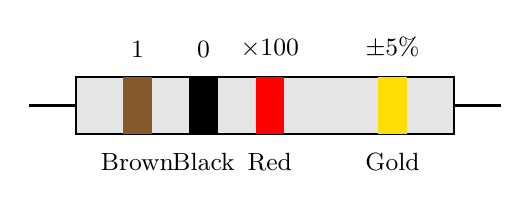
\begin{tikzpicture}[scale=1.2]
    % Resistor body
    \draw[thick, fill=gray!20] (0,0) rectangle (4,0.6);
    
    % Color bands
    \fill[brown!70!black] (0.5,0) rectangle (0.8,0.6);
    \fill[black] (1.2,0) rectangle (1.5,0.6);
    \fill[red] (1.9,0) rectangle (2.2,0.6);
    \fill[yellow!80!orange] (3.2,0) rectangle (3.5,0.6);
    
    % Labels
    \node[below, font=\small] at (0.65,-0.1) {Brown};
    \node[below, font=\small] at (1.35,-0.1) {Black};
    \node[below, font=\small] at (2.05,-0.1) {Red};
    \node[below, font=\small] at (3.35,-0.1) {Gold};
    
    \node[above, font=\small] at (0.65,0.7) {1};
    \node[above, font=\small] at (1.35,0.7) {0};
    \node[above, font=\small] at (2.05,0.7) {\(\times 100\)};
    \node[above, font=\small] at (3.35,0.7) {\(\pm 5\%\)};
    
    % Leads
    \draw[thick] (-0.5,0.3) -- (0,0.3);
    \draw[thick] (4,0.3) -- (4.5,0.3);
\end{tikzpicture}
\caption{Resistor with Brown-Black-Red-Gold Color Bands}
\end{figure}

\begin{itemize}
    \item Band 1 (Brown): 1 (first digit)
    \item Band 2 (Black): 0 (second digit)
    \item Band 3 (Red): \(\times 10^2 = \times 100\) (multiplier)
    \item Band 4 (Gold): \(\pm 5\%\) (tolerance)
\end{itemize}

\[
R = (10) \times 100 = 1000\,\Omega = 1\,k\Omega \pm 5\%\]

\subparagraph{Tolerance Range:}
For 1\,k\(\Omega\) \(\pm\) 5\%: Minimum = \(1000 - 50 = 950\,\Omega\), Maximum = \(1000 + 50 = 1050\,\Omega\)

\paragraph{Five and Six-Band Codes:}
For precision resistors, five or six bands are used where the first three bands represent significant digits, followed by multiplier, tolerance, and optionally temperature coefficient.

\paragraph{Reading Direction:}
The tolerance band (usually gold or silver) is slightly separated from other bands and should be on the right side when reading. Start reading from the opposite end.

\paragraph{Mnemonic:}
\emph{``BB ROY of Great Britain had a Very Good Wife: Black Brown Red Orange Yellow Green Blue Violet Grey White!''}

% ========================================
% QUESTION 1(c) OR: LDR-Light Dependent Resistor (7 marks)
% Demonstrates: Construction, working, characteristics, applications with diagram
% ========================================

\subsection{Question 1(c) OR [7 marks]}
\textbf{Explain construction, working, characteristic and application of LDR.}

\subsubsection{Solution}

A \textbf{Light Dependent Resistor (LDR)}, also called a photoresistor or photocell, is a passive semiconductor device whose resistance varies inversely with the intensity of light falling on it. It is widely used in light-sensing applications.

\paragraph{Construction:}

\begin{figure}[H]
\centering
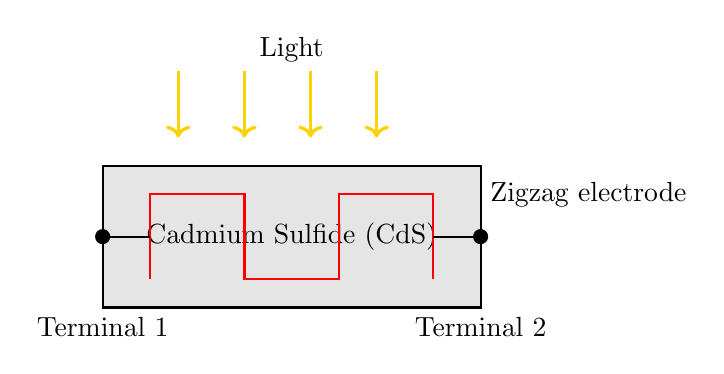
\begin{tikzpicture}[scale=1.2]
    % LDR body
    \draw[thick, fill=gray!20] (0,0) rectangle (4,1.5);
    \node at (2,0.75) {Cadmium Sulfide (CdS)};
    
    % Serpentine track
    \draw[thick, red] (0.5,0.3) -- (0.5,1.2) -- (1.5,1.2) -- (1.5,0.3) -- (2.5,0.3) -- (2.5,1.2) -- (3.5,1.2) -- (3.5,0.3);
    
    % Terminals
    \draw[thick] (0,0.75) -- (0.5,0.75);
    \draw[thick] (4,0.75) -- (3.5,0.75);
    \fill (0,0.75) circle (0.08);
    \fill (4,0.75) circle (0.08);
    
    % Light rays
    \foreach \x in {0.8,1.5,2.2,2.9}
        \draw[->,yellow!70!orange, very thick] (\x,2.5) -- (\x,1.8);
    \node[above] at (2,2.5) {Light};
    
    % Labels
    \node[below] at (0,0) {Terminal 1};
    \node[below] at (4,0) {Terminal 2};
    \node[right] at (4,1.2) {Zigzag electrode};
\end{tikzpicture}
\caption{LDR Construction}
\end{figure}

The LDR consists of a \textbf{semiconductor material} (typically Cadmium Sulfide - CdS or Cadmium Selenide - CdSe) deposited on a ceramic substrate. Two metal electrodes in a zigzag pattern are placed on the semiconductor surface to provide maximum contact area. The entire assembly is encapsulated in a transparent or semi-transparent casing to allow light to reach the sensitive material.

\paragraph{Working Principle:}

LDR operation is based on the \textbf{photoconductivity} phenomenon. In darkness, the semiconductor material has very high resistance (can be several megaohms) because there are few free charge carriers. When light photons strike the semiconductor surface, they impart energy to the electrons, causing them to break free from atoms and become \emph{free charge carriers}. This increases the conductivity and thus decreases the resistance. The resistance change is approximately logarithmic with light intensity.

\paragraph{VI Characteristics:}

The VI characteristic shows a linear relationship (Ohmic behavior) at constant light intensity. Different light levels produce different slopes, with higher light intensity producing steeper slopes (lower resistance). Under illuminated conditions, the LDR exhibits low resistance (few k\(\Omega\)), allowing larger current flow for a given voltage. In darkness, the resistance is very high (in M\(\Omega\) range), resulting in minimal current flow for the same voltage.

\paragraph{Key Specifications:}
\begin{description}
    \item[Dark Resistance:] 1\,M\(\Omega\) to 10\,M\(\Omega\) (typical)
    \item[Light Resistance:] Few hundred ohms to few k\(\Omega\)
    \item[Response Time:] Relatively slow (milliseconds), slower than photodiodes
    \item[Spectral Response:] Peak sensitivity in visible light spectrum (500-700\,nm for CdS)
\end{description}

\subparagraph{Temperature Effect:}
LDR resistance also varies slightly with temperature, which can introduce errors in precision applications.

\paragraph{Applications:}
\begin{itemize}
    \item \textbf{Automatic Street Lights:} Turn on/off based on ambient light
    \item \textbf{Light Meters:} In cameras and photography equipment
    \item \textbf{Burglar Alarms:} Detect beam interruption
    \item  \textbf{Solar Tracking Systems:} Optimize solar panel orientation
    \item \textbf{Display Brightness Control:} Adjust screen brightness automatically
\end{itemize}

\paragraph{Mnemonic:}
\emph{``LDR: Light Decreases Resistance -- More light, Less resistance!''}


% ========================================
% QUESTION 2(a): Classify Resistors Based on Materials (3 marks)
% ========================================

\section{Question 2}

\subsection{Question 2(a) [3 marks]}
\textbf{Classify Resistors based on materials.}

\subsubsection{Solution}

Resistors are classified based on the \textbf{resistive material} used in their construction. The material determines the resistor's characteristics such as stability, tolerance, temperature coefficient, power rating, and cost.

\paragraph{Classification Based on Materials:}
\begin{description}
    \item[Carbon Composition Resistors:] Made from a mixture of carbon particles and insulating binder. Inexpensive but have poor stability and high temperature coefficient. Tolerance typically \(\pm 5\%\) to \(\pm 20\%\).
    \item[Carbon Film Resistors:] Made by depositing a thin carbon film on a ceramic rod. Better stability than carbon composition, lower noise, tolerance \(\pm 2\%\) to \(\pm 5\%\).
    \item[Metal Film Resistors:] Made by depositing a thin metal (usually nickel-chromium) film on ceramic substrate. Excellent stability, low temperature coefficient, tight tolerances (\(\pm 0.1\%\) to \(\pm 2\%\)), used in precision circuits.
    \item[Wire-Wound Resistors:] Made by winding resistance wire (nichrome, manganin) on ceramic core. High power handling capability, very stable, used in power applications. Can have inductive effects at high frequencies.
    \item[Metal Oxide Resistors:] Made from metal oxide film deposited on ceramic core. Excellent high-temperature stability, used in applications requiring high reliability.
\end{description}

\paragraph{Mnemonic:}
\emph{``CCMWM: Carbon, Carbon-film, Metal-film, Wire-wound, Metal-oxide -- Materials Make Resistors!''}

% ========================================
% QUESTION 2(b): Calculate Resistor Values (4 marks)
% ========================================

\subsection{Question 2(b) [4 marks]}
\textbf{Calculate value of resistor for a given color code. (i) Brown, Black, Yellow, Golden (ii) Yellow, Violet, Red, Silver}

\subsubsection{Solution}

Using the standard resistor color code, we calculate the resistance value for each given color combination.

\paragraph{(i) Brown, Black, Yellow, Golden:}

\begin{itemize}
    \item Band 1 (Brown): 1 (first digit)
    \item Band 2 (Black): 0 (second digit)
    \item Band 3 (Yellow): \(\times 10^4\) (multiplier)
    \item Band 4 (Golden): \(\pm 5\%\) (tolerance)
\end{itemize}

\[
R_1 = (10) \times 10^4 = 100{,}000\,\Omega = 100\,k\Omega \pm 5\%
\]

\subparagraph{Tolerance Range:}
Minimum = \(100{,}000 - 5{,}000 = 95{,}000\,\Omega = 95\,k\Omega\)

Maximum = \(100{,}000 + 5{,}000 = 105{,}000\,\Omega = 105\,k\Omega\)

\paragraph{(ii) Yellow, Violet, Red, Silver:}

\begin{itemize}
    \item Band 1 (Yellow): 4 (first digit)
    \item Band 2 (Violet): 7 (second digit)
    \item Band 3 (Red): \(\times 10^2\) (multiplier)
    \item Band 4 (Silver): \(\pm 10\%\) (tolerance)
\end{itemize}

\[
R_2 = (47) \times 10^2 = 4{,}700\,\Omega = 4.7\,k\Omega \pm 10\%
\]

\subparagraph{Tolerance Range:}
Minimum = \(4{,}700 - 470 = 4{,}230\,\Omega = 4.23\,k\Omega\)

Maximum = \(4{,}700 + 470 = 5{,}170\,\Omega = 5.17\,k\Omega\)

\paragraph{Summary:}
\begin{description}
    \item[Resistor 1:] \(100\,k\Omega \pm 5\%\) (range: 95k\(\Omega\) to 105k\(\Omega\))
    \item[Resistor 2:] \(4.7\,k\Omega \pm 10\%\) (range: 4.23k\(\Omega\) to 5.17k\(\Omega\))
\end{description}

\paragraph{Mnemonic:}
\emph{``Read Band 1-2 as digits, Band 3 adds zeros, Band 4 shows tolerance!''}

% ========================================
% QUESTION 2(c): Electrolytic Capacitor Construction (7 marks)
% ========================================

\subsection{Question 2(c) [7 marks]}
\textbf{Illustrate construction and operation of Electrolytic capacitors.}

\subsubsection{Solution}

\textbf{Electrolytic capacitors} are polarized capacitors that use an electrolyte as one of the plates and an oxide layer as the dielectric. They provide very high capacitance values in compact sizes, making them essential in power supply circuits.

\paragraph{Construction:}

\begin{figure}[H]
\centering
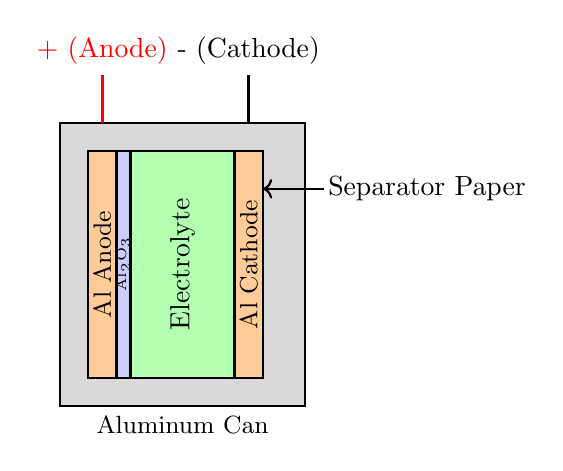
\begin{tikzpicture}[scale=1.2]
    % Outer casing
    \draw[thick, fill=gray!30] (-0.3,-1.5) rectangle (2.3,1.5);
    
    % Anode foil (aluminum)
    \draw[thick, fill=orange!40] (0,-1.2) rectangle (0.3,1.2);
    \node[rotate=90, font=\small] at (0.15,0) {Al Anode};
    
    % Oxide layer (dielectric)
    \draw[thick, fill=blue!20] (0.3,-1.2) rectangle (0.45,1.2);
    \node[rotate=90, font=\tiny] at (0.375,0) {Al\(_2\)O\(_3\)};
    
    % Electrolyte
    \draw[thick, fill=green!30] (0.45,-1.2) rectangle (1.55,1.2);
    \node[rotate=90] at (1,0) {Electrolyte};
    
    % Cathode foil
    \draw[thick, fill=orange!40] (1.55,-1.2) rectangle (1.85,1.2);
    \node[rotate=90, font=\small] at (1.7,0) {Al Cathode};
    
    % Terminals
    \draw[very thick, red] (0.15,1.5) -- (0.15,2) node[above] {+ (Anode)};
    \draw[very thick] (1.7,1.5) -- (1.7,2) node[above] {- (Cathode)};
    
    % Labels
    \node[below, font=\small] at (1,-1.5) {Aluminum Can};
    \draw[->, thick] (2.5,0.8) -- (1.85,0.8) node[right, xshift=0.7cm] {Separator Paper};
\end{tikzpicture}
\caption{Electrolytic Capacitor Cross-Section}
\end{figure}

\paragraph{Key Components:}
\begin{description}
    \item[Anode Foil:] Aluminum foil that is electrochemically etched to increase surface area. Positive Terminal.
    \item[Dielectric Layer:] Thin aluminum oxide (Al\(_2\)O\(_3\)) layer formed on anode surface through anodization. Thickness typically 1-10\,nm, providing very high capacitance.
    \item[Electrolyte:] Liquid, gel, or solid electrolyte serves as the actual cathode (negative plate). Maintains ionic conduction and reforms oxide layer.
    \item[Cathode Foil:] Second aluminum foil in contact with electrolyte, connected to negative terminal.
    \item[Separator:] Porous paper soaked in electrolyte, prevents direct contact between anode and cathode.
    \item[Casing:] Aluminum can enclosing the entire assembly with safety vent.
\end{description}

\paragraph{Operation Principle:}

The capacitance is determined by the oxide layer thickness and surface area. When DC voltage is applied with correct polarity, the oxide layer acts as dielectric. The very thin oxide layer (\(\sim\)1.4\,nm per volt) and large anode surface area yield high capacitance values (typically 1\,\(\mu\)F to 10{,}000\,\(\mu\)F or more).

\subparagraph{Capacitance Formula:}
\[
C = \frac{\epsilon_0 \epsilon_r A}{d}
\]
Where \(\epsilon_r \approx 8-10\) for Al\(_2\)O\(_3\), \(A\) is large due to etching, \(d\) is very small (oxide thickness).

\paragraph{Important Characteristics:}
\begin{itemize}
    \item \textbf{Polarity:} MUST be connected with correct polarity. Reverse voltage damages oxide layer causing failure or explosion.
    \item \textbf{High Capacitance:} Values from 1\,\(\mu\)F to several farads in small package.
    \item \textbf{Voltage Rating:} Typically 6.3V to 450V. Never exceed rated voltage.
    \item \textbf{ESR (Equivalent Series Resistance):} Affects ripple current capability and heating.
    \item \textbf{Leakage Current:} Small DC current flows through dielectric, which is normal but increases with age and temperature.
    \item \textbf{Self-Healing:} Can reform oxide layer to some extent if voltage is slowly applied after storage.
\end{itemize}

\subparagraph{Failure Modes:}
Reverse polarity, overvoltage, overheating, or aging can cause electrolyte evaporation, oxide breakdown, or pressure buildup leading to vent activation or catastrophic failure.

\paragraph{Applications:}
\begin{enumerate}
    \item \textbf{Power Supply Filtering:} Smoothing rectified AC in DC power supplies
    \item \textbf{Coupling/Decoupling:} Blocking DC while passing AC signals
    \item \textbf{Energy Storage:} In camera flashes, audio amplifiers, motor starting circuits
    \item \textbf{Timing Circuits:} Where large time constants are needed
\end{enumerate}

\paragraph{Mnemonic:}
\emph{``ELECTROLYTIC: Etched anode, Large capacitance, Electrolyte cathode, Correct Polarity, Thin Oxide dielectric, Liquid inside, aloYed for high-C, Thin layer yields high capacitance, Ionically conducting, Can explode if reversed!''}


% ========================================
% QUESTION 3(a): Filter Circuit Importance (3 marks)
% Section starting from Question paper line 36
% ========================================

\section{Question 3}

\subsection{Question 3(a) [3 marks]}
\textbf{State the importance of filter circuit in rectifier.}

\subsubsection{Solution}

A \textbf{filter circuit} is an essential component in rectifier systems that smooths the pulsating DC output from the rectifier into a steady DC voltage suitable for electronic circuits. Without filtering, the rectified output contains significant AC ripple components that can damage sensitive electronic components.

\paragraph{Importance of Filter Circuits:}
\begin{description}
    \item[Ripple Reduction:] Removes AC components from pulsating DC, providing smooth DC output. Reduces ripple factor from 1.21 (half-wave) or 0.48 (full-wave) to near zero.
    \item[Voltage Regulation:] Maintains relatively constant DC voltage despite variations in load current or input AC voltage.
    \item[Circuit Protection:] Prevents AC ripple from damaging sensitive electronic components like ICs, transistors, and operational amplifiers that require pure DC.
    \item[Improved Efficiency:] Enables efficient power transfer by minimizing power loss in AC ripple components.
    \item[Noise Reduction:] Reduces electrical noise and hum in audio and communication equipment caused by ripple voltage.
\end{description}

\paragraph{Mnemonic:}
\emph{``FILTER: Flatten ripples, Improve voltage stability, Less noise, Tame pulsations, Enable smooth DC, Regulate power!''}

% ========================================
% QUESTION 3(b): P-type vs N-type Semiconductors (4 marks)
% ========================================

\subsection{Question 3(b) [4 marks]}
\textbf{Differentiate between P type semiconductor and N type semiconductor.}

\subsubsection{Solution}

Semiconductors are classified as \textbf{P-type} and \textbf{N-type} based on the type of doping impurity added to intrinsic (pure) semiconductor material.

\begin{table}[H]
\centering
\caption{P-type vs N-type Semiconductor Comparison}
\begin{tabularx}{\textwidth}{lXX}
\toprule
\textbf{Parameter} & \textbf{P-type Semiconductor} & \textbf{N-type Semiconductor} \\
\midrule
Doping & Trivalent impurity (Boron, Gallium, Indium) & Pentavalent impurity (Phosphorus, Arsenic, Antimony) \\
Majority Carriers & Holes (positive charge carriers) & Electrons (negative charge carriers) \\
Minority Carriers & Electrons & Holes \\
Charge & Electrically neutral overall & Electrically neutral overall \\
Conductivity & Increases with hole concentration & Increases with electron concentration \\
Energy Level & Acceptor energy level near valence band & Donor energy level near conduction band \\
Symbol & P & N \\
\bottomrule
\end{tabularx}
\end{table}

\paragraph{P-type Formation:}
When trivalent impurity (3 valence electrons) is added to silicon (4 valence electrons), it creates a \emph{hole} or vacancy in the covalent bond structure. These holes act as positive charge carriers. The impurity atoms are called \textbf{acceptors} because they accept electrons.

\paragraph{N-type Formation:}
When pentavalent impurity (5 valence electrons) is added to silicon (4 valence electrons), the extra electron becomes a free charge carrier. These free electrons conduct current. The impurity atoms are called \textbf{donors} because they donate electrons.

\subparagraph{Key Point:}
Both remain electrically neutral because the number of protons equals the number of electrons in the overall structure.

\paragraph{Mnemonic:}
\emph{``P: Positive holes from  Trivalent; N: Negative electrons from Pentavalent!''}

% ========================================
% QUESTION 3(c): Bridge Rectifier with Waveforms (7 marks)
% ========================================

\subsection{Question 3(c) [7 marks]}
\textbf{Illustrate working of Bridge Rectifier with waveforms.}

\subsubsection{Solution}

A \textbf{bridge rectifier} is a full-wave rectifier circuit that uses four diodes in a bridge configuration to convert AC voltage to pulsating DC. It utilizes both half-cycles of the input AC waveform, providing better efficiency than half-wave rectifiers.

\paragraph{Circuit Diagram:}

\begin{figure}[H]
\centering
\begin{circuitikz}[scale=1.3]
    % AC Source
    \draw (0,0) to[sV, l=\(V_{in}\)] (0,3);
    
    % Bridge diodes
    \draw (0,3) -- (2,3);
    \draw (2,3) to[D*, l=\(D_1\)] (4,3);
    \draw (4,3) -- (6,3);
    \draw (6,3) to[D*, l=\(D_2\)] (6,1.5);
    
    \draw (0,0) -- (2,0);
    \draw (2,0) to[D*, l=\(D_4\)] (4,0);
    \draw (4,0) -- (6,0);
    \draw (6,0) to[D*, l_=\(D_3\)] (6,1.5);
    
    % Load resistor
    \draw (6,1.5) to[R, l=\(R_L\)] (6,1.5);
    \draw (6,3) -- (7,3) node[above] {\(+\)};
    \draw (6,0) -- (7,0) node[below] {\(-\)};
    
    % Output voltage
    \draw[<->] (7.5,3) -- (7.5,0) node[midway, right] {\(V_{out}\)};
\end{circuitikz}
\caption{Bridge Rectifier Circuit}
\end{figure}

\paragraph{Working Principle:}

The bridge rectifier operates in two half-cycles:

\subparagraph{Positive Half-Cycle:}
When the AC input is positive (top terminal positive, bottom terminal negative), diodes \(D_1\) and \(D_3\) are forward-biased and conduct, while \(D_2\) and \(D_4\) are reverse-biased and block. Current path: AC source \(\rightarrow\) \(D_1\) \(\rightarrow\) Load \(R_L\) \(\rightarrow\) \(D_3\) \(\rightarrow\) AC source. Output voltage appears across load.

\subparagraph{Negative Half-Cycle:}
When the AC input is negative (top terminal negative, bottom terminal positive), diodes \(D_2\) and \(D_4\) are forward-biased and conduct, while \(D_1\) and \(D_3\) are reverse-biased and block. Current path: AC source \(\rightarrow\) \(D_2\) \(\rightarrow\) Load \(R_L\) \(\rightarrow\) \(D_4\) \(\rightarrow\) AC source. Output voltage appears with same polarity across load.

\paragraph{Waveforms:}

\begin{figure}[H]
\centering
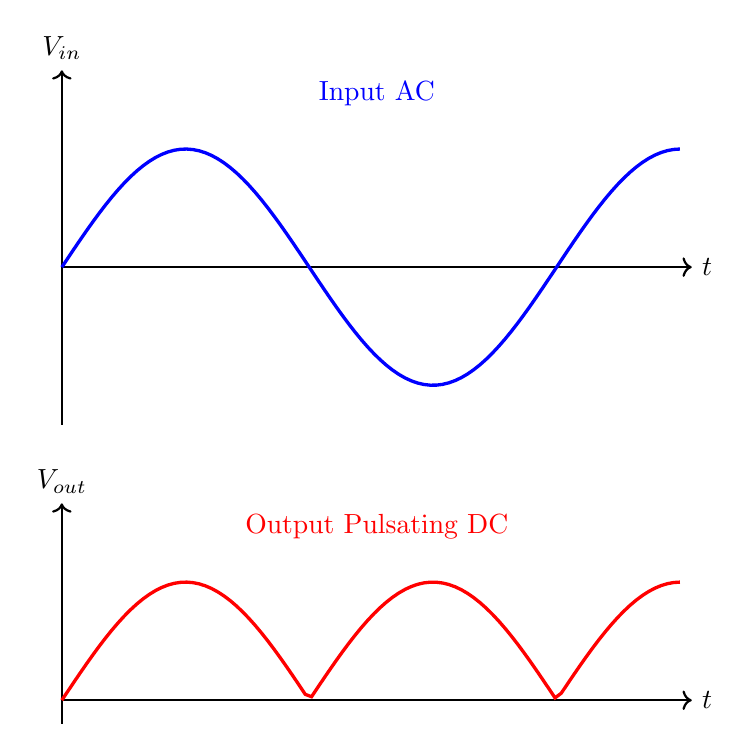
\begin{tikzpicture}[scale=1.0]
    % Input AC waveform
    \draw[->, thick] (0,0) -- (8,0) node[right] {\(t\)};
    \draw[->, thick] (0,-2) -- (0,2.5) node[above] {\(V_{in}\)};
    \draw[blue, very thick] plot[domain=0:7.85, samples=100] (\x, {1.5*sin(\x r)});
    \node[blue] at (4,2.2) {Input AC};
    
    % Output waveform
    \begin{scope}[yshift=-5.5cm]
        \draw[->, thick] (0,0) -- (8,0) node[right] {\(t\)};
        \draw[->, thick] (0,-0.3) -- (0,2.5) node[above] {\(V_{out}\)};
        \draw[red, very thick] plot[domain=0:7.85, samples=100] (\x, {1.5*abs(sin(\x r))});
        \node[red] at (4,2.2) {Output Pulsating DC};
    \end{scope}
\end{tikzpicture}
\caption{Bridge Rectifier Input and Output Waveforms}
\end{figure}

\paragraph{Key Parameters:}
\begin{description}
    \item[Efficiency:] \(\eta = 81.2\%\) (theoretical maximum, double that of half-wave)
    \item[Ripple Factor:] \(r = 0.48\) (much lower than half-wave 1.21)
    \item[Peak Inverse Voltage (PIV):] \(PIV = V_m\) (each diode must withstand peak AC voltage)
    \item[DC Output:] \(  V_{DC} = \frac{2V_m}{\pi} = 0.636 V_m\) (double that of half-wave)
    \item[Frequency:] Output ripple frequency is double the input AC frequency (100Hz for 50Hz input)
\end{description}

\paragraph{Advantages:}
\begin{itemize}
    \item No center-tapped transformer required (lower cost)
    \item Higher efficiency (81.2\%) compared to half-wave (40.6\%)
    \item Lower ripple factor (easier filtering)
    \item Better DC output voltage utilization
    \item Both half-cycles of AC are utilized
\end{itemize}

\paragraph{Disadvantages:}
\begin{itemize}
    \item Requires four diodes instead of one
    \item Two diodes conduct simultaneously, resulting in higher voltage drop (approximately 1.4V)
    \item Slightly more complex circuit than center-tapped full-wave rectifier
\end{itemize}

\subparagraph{Applications:}
Bridge rectifiers are widely used in power supplies for computers, mobile chargers, battery chargers, and industrial equipment due to their efficiency and simplicity.

\paragraph{Mnemonic:}
\emph{``BRIDGE: Both cycles used, Rectifies with Improved efficiency, Diodes in Groups of 2, Gives smoother output, Economical (no center-tap)!''}


% ========================================
% QUESTION 4, 5, and 6 - Continuing to complete all remaining questions
% ========================================

\section{Question 4}

\subsection{Question 4(a) [3 marks]}
\textbf{Define (1) PIV (2) Ripple Factor.}

\subsubsection{Solution}

\paragraph{(1) PIV - Peak Inverse Voltage:}

\textbf{Peak Inverse Voltage (PIV)} is the maximum reverse voltage that a diode in a rectifier circuit must withstand when it is reverse-biased during the non-conducting half-cycle. It represents the peak value of the AC voltage that appears across a non-conducting diode. Diodes must be rated to handle PIV to prevent breakdown. For half-wave rectifier PIV \(= V_m\), for center-tap full-wave PIV \(= 2V_m\), and for bridge rectifier PIV \(= V_m\), where \(V_m\) is peak AC voltage.

\paragraph{(2) Ripple Factor:}

\textbf{Ripple Factor (r)} is a measure of the effectiveness of a rectifier and filter circuit in converting AC to pure DC. It is defined as the ratio of RMS value of AC component to the DC component in the output. Mathematically:

\[
r = \frac{V_{ac}(rms)}{V_{dc}} = \frac{\sqrt{V_{rms}^2 - V_{dc}^2}}{V_{dc}}
\]

Lower ripple factor indicates better rectification and filtering. Ideal DC has \(r = 0\). Half-wave rectifier has \(r = 1.21\), full-wave rectifier has \(r = 0.48\).

\paragraph{Mnemonic:}
\emph{``PIV: Peak Inverse Voltage diodes must survive; Ripple: Ratio showing AC components alive!''}

\subsection{Question 4(b) [4 marks]}
\textbf{Illustrate VI characteristics of PN junction diode.}

\subsubsection{Solution}

The \textbf{Voltage-Current (VI) characteristic} of a PN junction diode shows the relationship between the voltage applied across the diode and the current flowing through it.

\begin{figure}[H]
\centering
\begin{tikzpicture}[scale=1.1]
    % Axes
    \draw[->] (-3,0) -- (3,0) node[right] {\(V\) (Voltage)};
    \draw[->] (0,-2) -- (0,3) node[above] {\(I\) (Current)};
    
    % Forward bias curve
    \draw[thick, blue, domain=0.6:2.4] plot (\x, {0.8*(\x-0.6)^2});
    
    % Reverse bias curve
    \draw[thick, red] (-2.5,-0.3) -- (-0.3,-0.3);
    
    % Breakdown
    \draw[thick, red] (-2.5,-0.3) -- (-2.5,-1.8);
    
    % Labels
    \node at (1.8,2.5) [blue] {Forward bias};
    \node at (-1.8,-0.6) [red] {Reverse bias};
    \node at (-2.2,-1.8) [red] {Breakdown};
    
    % Threshold voltage
    \draw[dashed] (0.7,0) -- (0.7,0.3);
    \node[below] at (0.7,-0.1) {\(V_{\gamma}\)};
    
    % Reverse saturation current
    \draw[dashed] (0,-0.3) -- (-0.5,-0.3);
    \node[left] at (-0.1,-0.3) {\(I_S\)};
\end{tikzpicture}
\caption{VI Characteristics of PN Junction Diode}
\end{figure}

\paragraph{Forward Bias Region:}
When positive terminal connected to P-side and negative to N-side, barrier potential decreases. Very small current flows until voltage exceeds threshold (\(V_{\gamma} \approx 0.7V\) for Si, 0.3V for Ge). Beyond threshold, current increases exponentially: \(I = I_S(e^{V/\eta V_T} - 1)\).

\paragraph{Reverse Bias Region:}
When positive terminal connected to N-side and negative to P-side, barrier potential increases. Very small reverse saturation current \(I_S\) (few \(\mu A\)) flows due to minority carriers. Remains nearly constant independent of reverse voltage.

\paragraph{Breakdown Region:}
At large reverse voltage, breakdown occurs due to avalanche or Zener effect. Current increases rapidly. This can damage regular diodes but is utilized in Zener diodes.

\paragraph{Mnemonic:}
\emph{``VI Curve: Forward voltage threshold, then Infinite current rise; Reverse gives tiny current, Breakdown at high reverse!''}

\subsection{Question 4(c) [7 marks]}
\textbf{Explain the working of capacitor input and choke input filter with waveforms.}

\subsubsection{Solution}

Filter circuits remove ripple from rectified output. Two common types are \textbf{capacitor input filter} and \textbf{choke input filter}.

\paragraph{Capacitor Input Filter:}

\subparagraph{Circuit and Working:}
A large capacitor is connected in parallel with the load. During the positive half-cycle when diode conducts, capacitor charges to peak voltage. When input drops, diode becomes reverse-biased and capacitor discharges through load, maintaining voltage. The capacitor repeatedly charges and discharges, providing relatively smooth DC.

\begin{figure}[H]
\centering
\begin{circuitikz}[scale=1.0]
    % Rectifier diode
    \draw (0,0) to[sV, l=\(V_{in}\)] (0,2);
    \draw (0,2) to[D, l=D] (3,2);
    
    % Capacitor
    \draw (3,2) to[short] (4,2);
    \draw (4,2) to[C, l=\(C\)] (4,0);
    
    % Load resistor
    \draw (4,2) to[short] (5.5,2);
    \draw (5.5,2) to[R, l=\(R_L\)] (5.5,0);
    
    % Ground
    \draw (0,0) -- (5.5,0);
    
    % Output voltage
    \draw[<->] (6,2) -- (6,0) node[midway, right] {\(V_{out}\)};
\end{circuitikz}
\caption{Capacitor Input Filter Circuit}
\end{figure}

\subparagraph{Waveform:}
Output voltage has small ripple riding on DC level. Ripple amplitude depends on capacitance and load resistance: \(V_{ripple} \approx \frac{I_{dc}}{fC}\) where \(f\) is ripple frequency.

\begin{figure}[H]
\centering
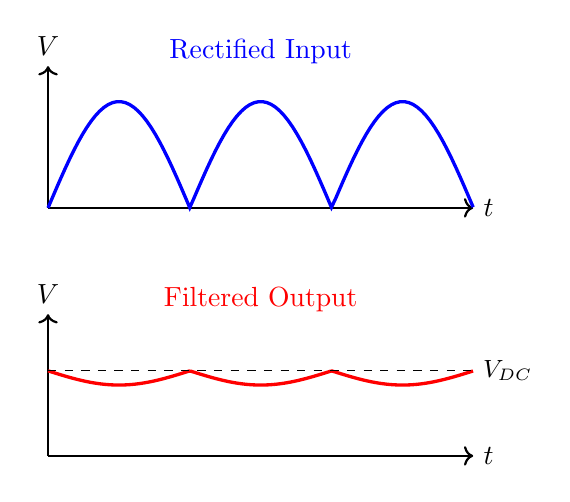
\begin{tikzpicture}[scale=0.9]
    % Input waveform
    \begin{scope}
        \draw[->, thick] (0,0) -- (6,0) node[right] {\(t\)};
        \draw[->,  thick] (0,0) -- (0,2) node[above] {\(V\)};
        \draw[blue, very thick] plot[domain=0:6, samples=100] (\x, {1.5*abs(sin(1.57*\x r))});
        \node[blue] at (3,2.2) {Rectified Input};
    \end{scope}
    
    % Output waveform with ripple
    \begin{scope}[yshift=-3.5cm]
        \draw[->, thick] (0,0) -- (6,0) node[right] {\(t\)};
        \draw[->, thick] (0,0) -- (0,2) node[above] {\(V\)};
        \draw[red, very thick] plot[domain=0:6, samples=200] (\x, {1.2 - 0.2*abs(sin(1.57*\x r))});
        \node[red] at (3,2.2) {Filtered Output};
        \draw[dashed] (0,1.2) -- (6,1.2) node[right, font=\small] {\(V_{DC}\)};
    \end{scope}
\end{tikzpicture}
\caption{Capacitor Filter Waveforms}
\end{figure}

\subparagraph{Characteristics:}
Good voltage regulation for light loads, poor for heavy loads. High peak diode current during charging. Used in low current applications. Ripple factor \(\approx \frac{1}{4\sqrt{3}fCR_L}\).

\paragraph{Choke Input Filter:}

\subparagraph{Circuit and Working:}
An inductor (choke) is connected in series with rectifier output, followed by a capacitor in parallel with load. The inductor opposes sudden changes in current due to its property \(V_L = L\frac{di}{dt}\). It smooths current variations. The capacitor then filters remaining ripple voltage.

\begin{figure}[H]
\centering
\begin{circuitikz}[scale=1.0]
    % Rectifier input
    \draw (0,0) to[sV, l=\(V_{in}\)] (0,2);
    \draw (0,2) to[D, l=D] (2,2);
    
    % Choke/Inductor
    \draw (2,2) to[L, l=\(L\)] (4,2);
    
    % Capacitor
    \draw (4,2) to[short] (5, 2);
    \draw (5,2) to[C, l=\(C\)] (5,0);
    
    % Load resistor
    \draw (5,2) to[short] (6.5,2);
    \draw (6.5,2) to[R, l=\(R_L\)] (6.5,0);
    
    % Ground
    \draw (0,0) -- (6.5,0);
    
    % Output voltage
    \draw[<->] (7,2) -- (7,0) node[midway, right] {\(V_{out}\)};
\end{circuitikz}
\caption{Choke (LC) Input Filter Circuit}
\end{figure}

\subparagraph{Waveform:}
Output voltage is very smooth with minimal ripple. The L-C combination provides excellent filtering.

\subparagraph{Characteristics:}
Better voltage regulation under varying loads. Lower peak diode current. Used in high current applications. Requires larger, heavier, expensive inductor. Ripple factor \(\approx \frac{R_L}{3\sqrt{2}\omega L}\) for L filter.

\paragraph{Comparison:}
\begin{description}
    \item[Capacitor Filter:] Simple, inexpensive, good for low current. Poor regulation at high currents. High peak diode current.
    \item[Choke Filter:] Better regulation, good for high current. More expensive, bulky. Lower peak diode current.
\end{description}

\paragraph{Mnemonic:}
\emph{``CAP filter: Charges quickly, Acts for light loads, Peak current high; CHOKE filter: Current smoothing, Heavy-duty, Opposes changes, Keeps regulation, Expensive but effective!''}

\section{Question 5}

\subsection{Question 5(a) [3 marks]}
\textbf{State the function and importance of Zener diode.}

\subsubsection{Solution}

A \textbf{Zener diode} is a special-purpose diode designed to operate in the reverse breakdown region safely and reliably. Its primary function is \textbf{voltage regulation}.

\paragraph{Function:}
When forward-biased, Zener diode behaves like a normal diode. When reverse-biased beyond its \textbf{Zener breakdown voltage} (\(V_Z\)), it maintains a nearly constant voltage across its terminals despite changes in current. This property makes it ideal for voltage regulation.

\paragraph{Importance:}
\begin{description}
    \item[Voltage Regulation:] Maintains constant output voltage despite input voltage or load current variations. Essential in power supplies.
    \item[Voltage Reference:] Provides stable reference voltage for measurement circuits, ADCs, and precision applications.
    \item[Over-voltage Protection:] Protects sensitive circuits by clipping excess voltage.
    \item[Wave Shaping:] Used in clipper and clamper circuits to modify waveform shapes.
    \item[Meter Protection:] Protects analog meters from over-voltage damage.
\end{description}

\paragraph{Mnemonic:}
\emph{``ZENER: Zero variation in voltage, Excellent for regulation, Needs reverse bias, Essential reference, Reliable protection!''}

\subsection{Question 5(b) [4 marks]}
\textbf{Describe Light emitting diode (LED) with its characteristic.}

\subsubsection{Solution}

A \textbf{Light Emitting Diode (LED)} is a PN junction diode that emits light when forward-biased. It converts electrical energy directly into light energy through electroluminescence.

\paragraph{Working Principle:}
When forward current flows through LED, electrons from N-region recombine with holes in P-region at the junction. During recombination, energy is released in the form of photons (light). The color of emitted light depends on the semiconductor material and energy band gap.

\paragraph{Materials and Colors:}
\begin{description}
    \item[Red:] Gallium Arsenide Phosphide (GaAsP), \(E_g \approx 1.8\ eV\)
    \item[Green:] Gallium Phosphide (GaP), \(E_g \approx 2.2\ eV\)
    \item[Blue:] Gallium Nitride (GaN), \(E_g \approx 2.9\ eV\)
    \item[White:] Blue LED with yellow phosphor coating or RGB combination
\end{description}

\paragraph{VI Characteristics:}
Similar to regular diode but with higher forward voltage drop (\(V_f \approx 1.8-3.5V\) depending on color). Current must be limited using series resistor. LED does not emit light in reverse bias. Typical operating current: 10-20\,mA.

\paragraph{Advantages:}
Low power consumption, long life (50{,}000+ hours), fast switching, compact size, available in various colors, no warm-up time, robust, environmentally friendly (no mercury).

\paragraph{Applications:}
Indicator lights, displays (seven-segment, dot matrix), backlighting, traffic signals, automotive lighting, general illumination, optical communication.

\paragraph{Mnemonic:}
\emph{``LED: Light from Energy released During electron-hole recombination!''}

\subsection{Question 5(c) [7 marks]}
\textbf{Illustrate the function of Zener diode as a voltage regulator.}

\subsubsection{Solution}

A \textbf{Zener diode voltage regulator} maintains constant output voltage despite variations in input voltage or load current. It operates in the reverse breakdown region where voltage remains nearly constant.

\paragraph{Basic Zener Regulator Circuit:}

\begin{figure}[H]
\centering
\begin{circuitikz}[scale=1.2]
    % Input voltage
    \draw (0,0) to[V, l=\(V_{in}\)] (0,3);
    
    % Series resistor
    \draw (0,3) to[R, l=\(R_S\)] (3,3);
    
    % Zener diode
    \draw (3,3) to[zzD, l=\(V_Z\)] (3,0);
    
    % Load resistor
    \draw (3,3) -- (5,3);
    \draw (5,3) to[R, l=\(R_L\)] (5,0);
    
    % Ground
    \draw (0,0) -- (5,0);
    
    % Output voltage
    \draw[<->] (5.5,3) -- (5.5,0) node[midway, right] {\(V_{out} = V_Z\)};
\end{circuitikz}
\caption{Zener Diode Voltage Regulator}
\end{figure}

\paragraph{Working Principle:}

The series resistor \(R_S\) and Zener diode act as a voltage divider. When \(V_{in} > V_Z\), Zener operates in breakdown region, maintaining \(V_{out} = V_Z\). The series resistor \(R_S\) drops the excess voltage:

\[
V_{R_S} = V_{in} - V_Z
\]

Current through \(R_S\):
\[
I_S = \frac{V_{in} - V_Z}{R_S} = I_Z + I_L
\]

where \(I_Z\) is Zener current and \(I_L\) is load current.

\paragraph{Line Regulation:}
When \(V_{in}\) increases, more current flows through \(R_S\). Zener conducts additional current to maintain constant \(V_Z\). Output remains stable.

\paragraph{Load Regulation:}
When load current \(I_L\) increases, Zener current \(I_Z\) decreases proportionally to maintain total current through \(R_S\) approximately constant. Output voltage remains at \(V_Z\) as long as \(I_Z\) stays above minimum holding current.

\paragraph{Design Considerations:}
\begin{itemize}
    \item Choose Zener voltage \(V_Z\) equal to desired output voltage
    \item \(V_{in(min)} > V_Z + 2V\) (minimum overhead)
    \item \(R_S = \frac{V_{in} - V_Z}{I_Z + I_L}\)
    \item Zener power: \(P_Z = V_Z \times I_{Z(max)}\)
    \item Ensure \(I_{Z(min)} < I_Z < I_{Z(max)}\) for proper regulation
\end{itemize}

\paragraph{Limitations:}
Limited current capability, poor efficiency, output not adjustable, generates heat, ripple rejection limited.

\paragraph{Applications:}
Low power voltage regulation, reference voltage sources, over-voltage protection, bias voltage for transistors, meter protection circuits.

\paragraph{Mnemonic:}
\emph{``REGULATOR: Reverse breakdown region, Excess voltage dropped by Rs, Generates constant output, Utilized for stabilization, Load variations handled, Automatic current adjustment, Typical application in power supplies, Output equals Vz, Reliable for low power!''}

\section{Question 6}

\subsection{Question 6(a) [3 marks]}
\textbf{Discuss transistor in brief.}

\subsubsection{Solution}

A \textbf{transistor} is a three-terminal active semiconductor device that can amplify or switch electronic signals. It is the fundamental building block of modern electronic circuits.

\paragraph{Types:}
\begin{description}
    \item[BJT (Bipolar Junction Transistor):] Uses both electrons and holes. Two types: NPN and PNP. Three regions: Emitter, Base, Collector.
    \item[FET (Field Effect Transistor):] Uses electric field to control current. Types include JFET and MOSFET. Three terminals: Source, Gate, Drain.
\end{description}

\paragraph{Functions:}
\begin{description}
    \item[Amplification:] Small input signal controls large output signal. Power, voltage, or current amplification.
    \item[Switching:] Acts as electronic switch - ON (saturation) or OFF (cutoff). Used in digital circuits, power control.
\end{description}

\paragraph{BJT Operating Regions:}
Cutoff (both junctions reverse-biased, transistor OFF), Active (EB forward, CB reverse, amplification), Saturation (both junctions forward, transistor fully ON).

\paragraph{Mnemonic:}
\emph{``TRANSISTOR: Three terminals, Amplifies or switches, Needs biasing, Silicon-based, Integrated everywhere, Semiconductor device, Two junction device, Output controlled by input, Revolutionized electronics!''}

\subsection{Question 6(b) [4 marks]}
\textbf{Derive relation between \(\alpha\) and \(\beta\) for transistor amplifier.}

\subsubsection{Solution}

In a transistor, \textbf{\(\alpha\)} (alpha) and \textbf{\(\beta\)} (beta) are current gain parameters that relate emitter, base, and collector currents.

\paragraph{Definition of \(\alpha\) (Common Base Current Gain):}
\[
\alpha = \frac{I_C}{I_E}
\]
Ratio of collector current to emitter current. Typically \(\alpha \approx 0.95\) to 0.99.

\paragraph{Definition of \(\beta\) (Common Emitter Current Gain):}
\[
\beta = \frac{I_C}{I_B}
\]
Ratio of collector current to base current. Typically \(\beta \approx 50\) to 300.

\paragraph{Derivation:}
Applying Kirchhoff's Current Law at transistor node:
\[
I_E = I_B + I_C
\]

From definition of \(\alpha\):
\[
I_C = \alpha I_E = \alpha(I_B + I_C)
\]

Expanding:
\[
I_C = \alpha I_B + \alpha I_C
\]

Rearranging:
\[
I_C - \alpha I_C = \alpha I_B
\]

\[
I_C(1 - \alpha) = \alpha I_B
\]

\[
\frac{I_C}{I_B} = \frac{\alpha}{1 - \alpha}
\]

Since \(\beta = \frac{I_C}{I_B}\):

\[
\boxed{\beta = \frac{\alpha}{1 - \alpha}}
\]

Similarly, solving for \(\alpha\):
\[
\beta(1 - \alpha) = \alpha
\]

\[
\beta - \beta\alpha = \alpha
\]

\[
\beta = \alpha + \beta\alpha = \alpha(1 + \beta)
\]

\[
\boxed{\alpha = \frac{\beta}{1 + \beta}}
\]

\paragraph{Numerical Example:}
If \(\alpha = 0.98\):
\[\beta = \frac{0.98}{1-0.98} = \frac{0.98}{0.02} = 49\]

If \(\beta = 100\):
\[\alpha = \frac{100}{1+100} = \frac{100}{101} = 0.99\]

\paragraph{Mnemonic:}
\emph{``Alpha over one-minus-alpha gives Beta; Beta over one-plus-beta gives Alpha!''}

\subsection{Question 6(c) [7 marks]}
\textbf{Explain in detail the construction of NPN and PNP transistor.}

\subsubsection{Solution}

\textbf{Bipolar Junction Transistors (BJTs)} are three-layer, two-junction semiconductor devices available in two configurations: \textbf{NPN} and \textbf{PNP}.

\paragraph{NPN Transistor Construction:}

\begin{figure}[H]
\centering
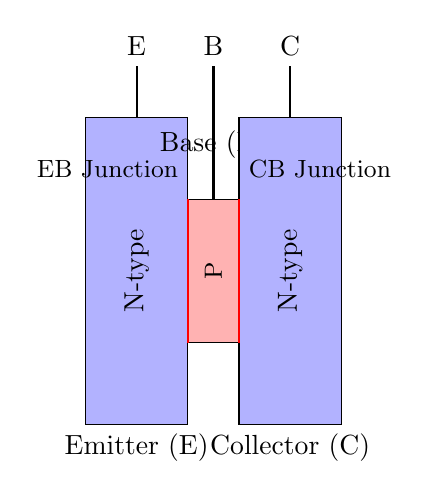
\begin{tikzpicture}[scale=1.3]
    % Layers
    \draw[fill=blue!30] (0,0) rectangle (1,3);
    \node at (0.5,1.5) [rotate=90] {N-type};
    \node[below] at (0.5,0) {Emitter (E)};
    
    \draw[fill=red!30] (1,0.8) rectangle (1.5,2.2);
    \node at (1.25,1.5) [rotate=90, font=\small] {P};
    \node[above] at (1.25,2.5) {Base (B)};
    
    \draw[fill=blue!30] (1.5,0) rectangle (2.5,3);
    \node at (2,1.5) [rotate=90] {N-type};
    \node[below] at (2,0) {Collector (C)};
    
    % Junctions
    \draw[thick, red] (1,0.8) -- (1,2.2);
    \node[left, font=\small] at (1,2.5) {EB Junction};
    \draw[thick, red] (1.5,0.8) -- (1.5,2.2);
    \node[right, font=\small] at (1.5,2.5) {CB Junction};
    
    % Terminals
    \draw[thick] (0.5,3) -- (0.5,3.5) node[above] {E};
    \draw[thick] (1.25,2.2) -- (1.25,3.5) node[above] {B};
    \draw[thick] (2,3) -- (2,3.5) node[above] {C};
\end{tikzpicture}
\caption{NPN Transistor Structure}
\end{figure}

\subparagraph{NPN Structure:}
\begin{description}
    \item[Emitter (N-type):] Heavily doped region that emits majority charge carriers (electrons). Moderate size, high conductivity.
    \item[Base (P-type):] Very thin (\(\sim 1\ \mu m\)) and lightly doped region between emitter and collector. Critical for transistor action.
    \item[Collector (N-type):] Moderately doped, largest region. Collects carriers from emitter through base.
\end{description}

\paragraph{PNP Transistor Construction:}

PNP transistor has opposite doping: P-type emitter, N-type base, P-type collector. Structure is mirror image of NPN.

\paragraph{Key Construction Features:}

\subparagraph{Base Region:}
Extremely thin to allow most carriers to diffuse across without recombination. Typical thickness 1-10\,\(\mu m\). Light doping ensures low recombination.

\subparagraph{Emitter Region:}
Heavily doped to inject maximum carriers. Doping concentration \(\approx 10^{19}\) atoms/cm\(^3\).

\subparagraph{Collector Region:}
Moderate doping, larger area than emitter to dissipate heat. Doping concentration \(\approx 10^{15}\) atoms/cm\(^3\).

\paragraph{Manufacturing Process:}
Uses techniques like diffusion, ion implantation, epitaxial growth on silicon wafer. Modern transistors fabricated as part of integrated circuits using photolithography.

\paragraph{Difference NPN vs PNP:}
\begin{description}
    \item[NPN:] Electrons are majority carriers. Current flows collector to emitter. Faster switching due to higher electron mobility.
    \item[PNP:] Holes are majority carriers. Current flows emitter to collector. Generally slower than NPN.
\end{description}

\paragraph{Symbol Convention:}
Arrow on emitter shows conventional current direction. NPN: arrow points outward (N to P). PNP: arrow points inward (P to N).

\paragraph{Mnemonic:}
\emph{``NPN: Not Pointing iN; PNP: Points iN Purposely!''}

\end{document}
